
%(BEGIN_QUESTION)
% Copyright 2008, Tony R. Kuphaldt, released under the Creative Commons Attribution License (v 1.0)
% This means you may do almost anything with this work of mine, so long as you give me proper credit

Predict how the operation of this operational amplifier circuit will be affected as a result of the following faults.  Consider each fault independently (i.e. one at a time, no coincidental faults):

$$\includegraphics[width=15.5cm]{i03269x01.eps}$$

\begin{itemize}
\item{} Resistor $R_1$ fails open:
\vskip 5pt
\item{} Solder bridge (short) across resistor $R_1$:
\vskip 5pt
\item{} Resistor $R_2$ fails open:
\vskip 5pt
\item{} Solder bridge (short) across resistor $R_2$:
\vskip 5pt
\item{} Broken wire between $R_1$/$R_2$ junction and inverting opamp input:
\end{itemize}

\vskip 10pt

For each of these conditions, explain {\it why} the resulting effects will occur.

\vskip 20pt \vbox{\hrule \hbox{\strut \vrule{} {\bf Suggestions for Socratic discussion} \vrule} \hrule}

\begin{itemize}
\item{} When performing fault analyses of opamp circuits, it is helpful to bear in mind the simplifying assumptions of negative-feedback opamp circuits.  Identify some of these assumptions, especially the one regarding input voltages to the opamp when negative feedback is in effect.
\end{itemize}

\underbar{file i03269}
%(END_QUESTION)





%(BEGIN_ANSWER)

\noindent
{\bf Partial answer:}

\medskip
%\item{} Resistor $R_1$ fails open: {\it $V_{out}$ = 0 volts.}
%\vskip 5pt
\item{} Solder bridge (short) across resistor $R_1$: {\it Output saturates negative.}
\vskip 5pt
%\item{} Resistor $R_2$ fails open: {\it Output saturates negative.}
%\vskip 5pt
%\item{} Solder bridge (short) across resistor $R_2$: {\it $V_{out}$ = 0 volts.}
%\vskip 5pt
\item{} Broken wire between $R_1$/$R_2$ junction and inverting opamp input: {\it Output voltage unpredictable.}
\end{itemize}

%(END_ANSWER)





%(BEGIN_NOTES)

\begin{itemize}
\item{} Resistor $R_1$ fails open: {\it $V_{out}$ = 0 volts.}
\vskip 5pt
\item{} Solder bridge (short) across resistor $R_1$: {\it Output saturates negative.}
\vskip 5pt
\item{} Resistor $R_2$ fails open: {\it Output saturates negative.}
\vskip 5pt
\item{} Solder bridge (short) across resistor $R_2$: {\it $V_{out}$ = 0 volts.}
\vskip 5pt
\item{} Broken wire between $R_1$/$R_2$ junction and inverting opamp input: {\it Output voltage unpredictable.}
\end{itemize}

The purpose of this question is to approach the domain of circuit troubleshooting from a perspective of knowing what the fault is, rather than only knowing what the symptoms are.  Although this is not necessarily a realistic perspective, it helps students build the foundational knowledge necessary to diagnose a faulted circuit from empirical data.  Questions such as this should be followed (eventually) by other questions asking students to identify likely faults based on measurements.

%INDEX% Electronics review: opamp inverting amplifier circuit

%(END_NOTES)


